\documentclass[handout]{beamer} %

 
\mode<presentation>
{
%\usetheme[titleprogressbar]{m}
  \usetheme{default}      % or try Darmstadt, Madrid, Warsaw, ...
  \usecolortheme{default} % or try albatross, beaver, crane, ...
  \usefonttheme{default}  % or try serif, structurebold, ...
  \setbeamertemplate{navigation symbols}{}
  \setbeamertemplate{caption}[numbered]
} 

\setbeamerfont{section in toc}{size=\Large}
\setbeamerfont{subsection in toc}{size=\large}
\addtobeamertemplate{navigation symbols}{}{%
    \usebeamerfont{footline}%
    \usebeamercolor[fg]{footline}%
    \hspace{1em}%
    \insertframenumber/\inserttotalframenumber
}

\usepackage{scrextend}

\usepackage[english]{babel}
\usepackage{color}
\usepackage[utf8x]{inputenc}
\usepackage{booktabs}
\usepackage{colortbl}
\usepackage{verbatim}
\usepackage{bm}
\usepackage{listings}
\usepackage{amsmath} 
\usepackage{hyperref}
\usepackage{array}
\usepackage{wasysym}
\usepackage{xmpmulti}
\usepackage{url}
%\newcounter{propCounter} 

\newtheorem{prop}{Proposition}
 \setbeamertemplate{theorems}[numbered]


\makeatletter
\renewenvironment{proof}[1][\proofname]{\par
  \pushQED{\qed}%
  \normalfont \topsep6\p@\@plus6\p@\relax
  \trivlist
  \item[\hskip\labelsep
        \itshape
    #1\@addpunct{.}]\mbox{} 
}{%
  \popQED\endtrivlist\@endpefalse
}
 
\newenvironment<>{proofs}[1][\proofname]{%
    \par
    \def\insertproofname{#1\@addpunct{.}}%
    \usebeamertemplate{proof begin}#2}
  {\usebeamertemplate{proof end}}
 \newenvironment<>{proofe}{%
    \par
    \pushQED{\qed}
    \setbeamertemplate{proof begin}{\begin{block}{}}
    \usebeamertemplate{proof begin}}
  {\popQED\usebeamertemplate{proof end}}

\makeatother




\def\blockSqz{\vspace*{-\baselineskip}\setlength\belowdisplayshortskip{0pt}}
\def\Put(#1,#2)#3{\leavevmode\makebox(0,0){\put(#1,#2){#3}}}
\usepackage{mathtools}
\hypersetup{colorlinks=false,linkcolor=green,pdfborderstyle={/S/U/W 1}}
\usepackage{tikz}
\def\checkmark{\tikz\fill[scale=0.4](0,.35) -- (.25,0) -- (1,.7) -- (.25,.15) -- cycle;} 
\usetikzlibrary{decorations.pathreplacing,calc}

\newcommand{\tikzmark}[2][-3pt]{\tikz[remember picture, overlay, baseline=-0.5ex]\node[#1](#2){};}

\tikzset{brace/.style={decorate, decoration={brace}},
 brace mirrored/.style={decorate, decoration={brace,mirror}},
}

\newcounter{brace}
\setcounter{brace}{0}
\newcommand{\drawbrace}[3][brace]{%
 \refstepcounter{brace}
 \tikz[remember picture, overlay]\draw[#1] (#2.center)--(#3.center)node[pos=0.5, name=brace-\thebrace]{};
}

\newcounter{arrow}
\setcounter{arrow}{0}
\newcommand{\drawcurvedarrow}[3][]{%
 \refstepcounter{arrow}
 \tikz[remember picture, overlay]\draw (#2.center)edge[#1]node[coordinate,pos=0.5, name=arrow-\thearrow]{}(#3.center);
}

% #1 options, #2 position, #3 text 
\newcommand{\annote}[3][]{%
 \tikz[remember picture, overlay]\node[#1] at (#2) {#3};
}
\usepackage{ellipsis} \renewcommand{\ellipsisgap}{0.05em}
\lstset{ 
  basicstyle=\ttfamily\footnotesize
}
\def\a{\alpha}
\def\dash{\text{ --- }}
\def\E{\mathbb{E}}
\def\one{\mathbf{1}}
\def\xit[#1]{{(x^{({#1})})}^T}%{(x^{(1)})}^T }
\DeclareMathOperator*{\argmin}{arg\!\min}
\DeclareMathOperator*{\argmax}{\arg\!\max} 
\usepackage{color} 
\usepackage{listings} 
\usepackage{setspace} 

\definecolor{Code}{rgb}{0,0,0} 
\definecolor{Decorators}{rgb}{0.5,0.5,0.5} 
\definecolor{Numbers}{rgb}{0.5,0,0} 
\definecolor{MatchingBrackets}{rgb}{0.25,0.5,0.5} 
\definecolor{Keywords}{rgb}{0,0,1} 
\definecolor{self}{rgb}{0,0,0} 
\definecolor{Strings}{rgb}{0,0.63,0} 
\definecolor{Comments}{rgb}{0,0.63,1} 
\definecolor{Backquotes}{rgb}{0,0,0} 
\definecolor{Classname}{rgb}{0,0,0} 
\definecolor{FunctionName}{rgb}{0,0,0} 
\definecolor{Operators}{rgb}{0,0,0} 
\definecolor{Background}{rgb}{0.98,0.98,0.98} 
 
\lstdefinelanguage{Python}{ 
numbers=left, 
numberstyle=\footnotesize, 
numbersep=1em, 
xleftmargin=1em, 
framextopmargin=2em, 
framexbottommargin=2em, 
showspaces=false, 
showtabs=false, 
showstringspaces=false, 
frame=l, 
tabsize=4, 
% Basic 
basicstyle=\ttfamily\small\setstretch{1}, 
backgroundcolor=\color{Background}, 
% Comments 
commentstyle=\color{Comments}\slshape, 
% Strings 
stringstyle=\color{Strings}, 
morecomment=[s][\color{Strings}]{"""}{"""}, 
morecomment=[s][\color{Strings}]{'''}{'''}, 
% keywords 
morekeywords={import,from,class,def,for,while,if,is,in,elif,else,not,and,or,print,break,continue,return,True,False,None,access,as,,del,except,exec,finally,global,import,lambda,pass,print,raise,try,assert}, 
keywordstyle={\color{Keywords}\bfseries}, 
% additional keywords 
morekeywords={[2]@invariant,pylab,numpy,np,scipy}, 
keywordstyle={[2]\color{Decorators}\slshape}, 
emph={self}, 
emphstyle={\color{self}\slshape}, 
% 
} 
\title[Learning From Data]{Learning From Data \\ Analysis on Programming Assignment 3 }

%\author{Shao-Lun Huang  \quad shaolun.huang@sz.tsinghua.edu.cn  }%\\
 %\smallskip
\author{ Feng Zhao  \quad zhaof17@mails.tsinghua.edu.cn}
%\institute{TBSI}
\date{12/11/2020}

\begin{document}
\setbeamertemplate{caption}{\raggedright\insertcaption\par}
\newcommand{\myalert}[1][]{\color{red} #1}
\begin{frame}
  \titlepage
\end{frame}



 % Uncomment these lines for an automatically generated outline.
 %\begin{frame}{Outline}
 % \tableofcontents
 %\end{frame}
 
 

\begin{frame}{KMeans Assumption}
\begin{block}{Problem}
	Without normalization, use kmeans to cluster the following data and analyze your unexpected result.
	\begin{figure}[!ht]
		\centering
		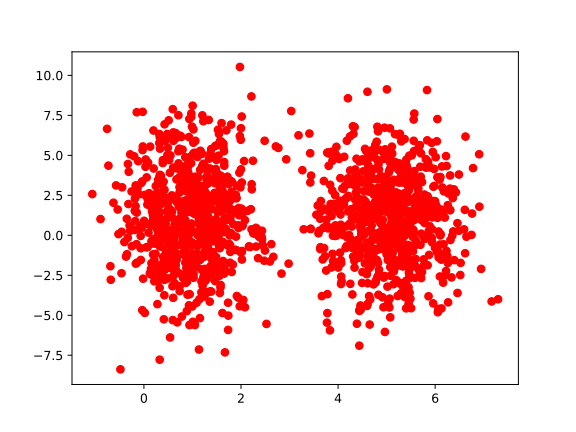
\includegraphics[width=6cm]{kmeans_data.png}
		\caption{data blob with two-ellipse contour}
	\end{figure}
\end{block}


\end{frame}
\begin{frame}{KMeans Assumption}
Using random initialization:
\begin{block}{Result}
	\begin{figure}[!ht]
	\centering
	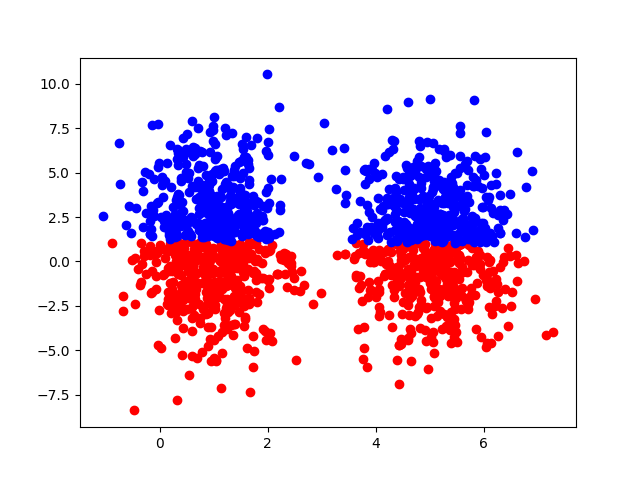
\includegraphics[width=6cm]{kmeans_result.png}
	\caption{unexpected clustering result with inertia equal to 11175}
\end{figure}
\end{block}
inertia of kmeans: 
$
\min_{C, \mu} \sum_{j=1}^k \sum_{x \in C_j}
|| x - \mu_j ||^2
$
\end{frame}

\begin{frame}{KMeans Assumption}
Choose the initial centroid of KMeans near \texttt{[1, 0], [5, 0]}:

\begin{figure}[!ht]
	\centering
	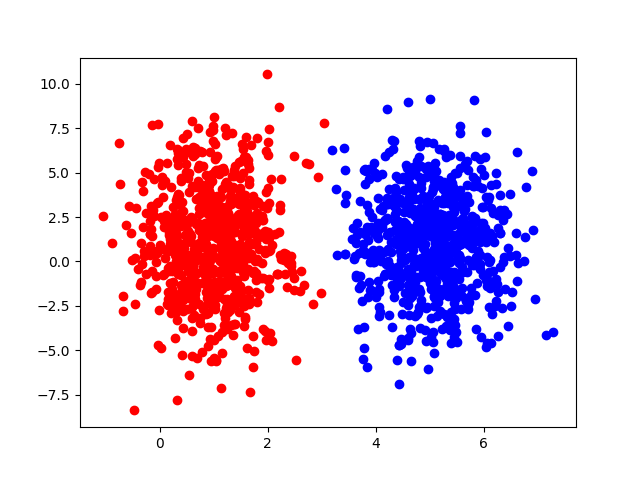
\includegraphics[width=6cm]{right_clustering.png}
	\caption{expected clustering result with inertia equal to 12771}	
\end{figure}

expected result is the local optima (\textbf{not} the global optima)
\end{frame}
\begin{frame}{KMeans Assumption}
Normalizing the data before using KMeans (RichardWilde1): \texttt{sklearn.preprocess.scale}

\begin{figure}[!ht]
	\centering
	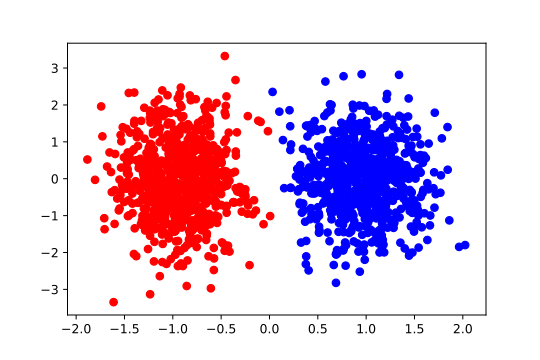
\includegraphics[width=6cm]{kmeans-clustering-normalized.png}
\end{figure}
\begin{itemize}
\item Major factor: unit variance assumption of KMeans
\item Minor factor: random initialization
\end{itemize}
\end{frame} 
\begin{frame}{Gaussian Kernel in Spectral Clustering}


\end{frame}

\end{document}
